\section{Gestione e struttura del database}
Una delle prime attività del progetto è stata la progettazione della base di
dati, e fin dall'inizio era chiaro che non si sarebbe trattato di uno schema
molto complesso. Infatti con sole tre tabelle si riesce a descrivere in modo
appropriato l'ambiente nel quale risiede il progetto.
\subsection{Schema Concettuale}
 La tabella principale e da cui si è partiti è
quella delle stazioni, che presenta una chiave primaria (Key), un nome con
cui è conosciuta, l'indirizzo cioè il nome della via nella quale risiede, la
posizione, formata da due coordinate geografiche di latitudine e longitudine che
sono realizzate mediante due variabili double, e
può ma non è costretta a possedere una descrizione formata da un testo. La
stazione possiede poi una Tipologia. Tramite colloquio con il commitente dott.
Marco  Aceti si è appreso come le stazioni di ricarica possono essere
raggruppate
in diversi insiemi dovuti al servizio vero e proprio che viene fornito oltre a
quello della ricarica. Esistono stazioni nelle quali è possibile noleggiare bici
elettriche e altre dove si può portare la propria bici per effettuare della manutenzione.
Dunque la tabella TipoStazione contiene per ogni riga una diversa tipologia di
stazione, formata dalla combinazione dei diversi servizi appena descritti, in
quanto ovviamente esistono negozi che propongono più servizi contemporaneamente.
Ogni istanza di questa tabella oltre a possedere una chiave che la identifica,
è caratterizzata dal nome (cioè la tipologia) e da un numero intero chiamato
Colore che viene utilizzato all'interno dell'applicazione per fornire un colore
diverso a ogni tipologia in modo da rendere più semplice agli utenti
l'identiticazione di ciò che può interessare loro. Nello schema deve poi essere
presente una tabella che tenga traccia degli utenti. Si presti attenzione che
questa tabella è diversa da quella gestita da Firebase relativa agli accessi e
alle tipologie di utenti descritta nel precedente capitolo: qui vengono presi in
considerazione il nome dell'utente e oltre alla chiave per identificarlo la
propria preferenza sulla tipologia di mappa scelta. Non si esclude che in futuro
si possano aggiungere ulteriori campi relativi a nuove preferenze che
potrebberero essere scelte. Nella figura \ref{schemaEr} è mostrato lo schema Entità-Relazione
del progetto. Si noti come una stazione debba per forza appartenere alla
relazione Inserimento in quanto deve essere stata inserita da qualcuno, ma un
utente può non appartenere a tale relazione in quanto può tranqullamente
utilizzare l'app per conoscere la posizioni di stazioni senza mai inserirne nessuna.

\begin{figure}[ht!]
    \centering
    {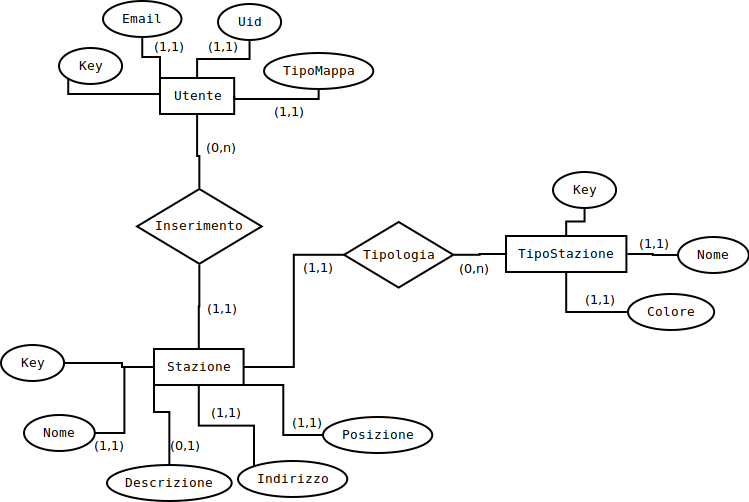
\includegraphics[scale=0.5]{ERTesi.png}\label{schemaEr}}
    \caption{Schema Concettuale del progetto}
\end{figure} 

\subsection{Schema Logico}
Data la semplicità dello schema Entità-Relazione la fase di progettazione logica
è stata anch'essa priva di ostacoli. Si è posta particolare attenzione alle
relazioni "Inserimento" e "Tipologia" perchè sarebbero potute diventare delle
tabelle ma dato che entrambe sono del tipo (1,1) verso (0,n) si è scelto di
renderle degli attributi della tabella Stazione, diventando quindi chiavi esterne. 

\begin{figure}[ht!]
    \centering
    {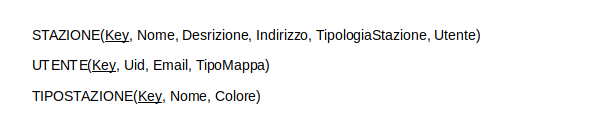
\includegraphics[scale=0.95]{LogicoTesi.png}\label{schemaLogico}}
    \caption{Schema Logico del progetto}
\end{figure} 

\subsection{Gestione dati in Firebase}